\section{Cumplimiento de requerimientos}
El en la sección \ref{sec:req-ana} se expusieron los requerimientos funcionales y no funcionales (secciones \ref{sec:req-fun} y \ref{sec:nonfunctional-req} respectivamente) para el sistema AutoSA. A continuación se exponen los cumplimientos de dichos requerimientos.

\subsection{Cumplimiento de requerimientos funcionales}
La sección \ref{sec:req-fun} lista los requerimientos funcionales del sistema AutoSA, de tales requerimientos se elaboraron los casos de uso, sección \ref{sec:casos-uso}, donde se describen los flujos que debe seguir el sistema AutoSA para cumplir con los requerimientos, es así que a continuación se expone que la implementación del sistema satisface los requerimientos funcionales junto con los casos de uso y muestra la operación del usuario.

\subsubsection{Automatización de los procesos en el Sistema de Abastecimiento}
Los requerimientos funcionales de las secciones \ref{sec:req-contestar} y \ref{sec:req-verificar} automatizan los procesos descritos en la sección \ref{sec:desc-general} y son reflejados en los casos de uso CU-CONTESTAAR y CU-VERIFICAR (ver secciones \ref{cu-contestar} y \ref{cu-verificar} respectivamente), la implementación es mostrada en la sección \ref{sec:agente}. El usuario puede ejecutar las automatizaciones desde la herramienta \textit{Sahi} de la siguiente forma:
\begin{itemize}
	\item Iniciar \textit{Sahi} sobre el explorar de Internet (ver punto 1 de la Figura \ref{fig:ss-sahi})
	\begin{figure}[h]
		\centering
		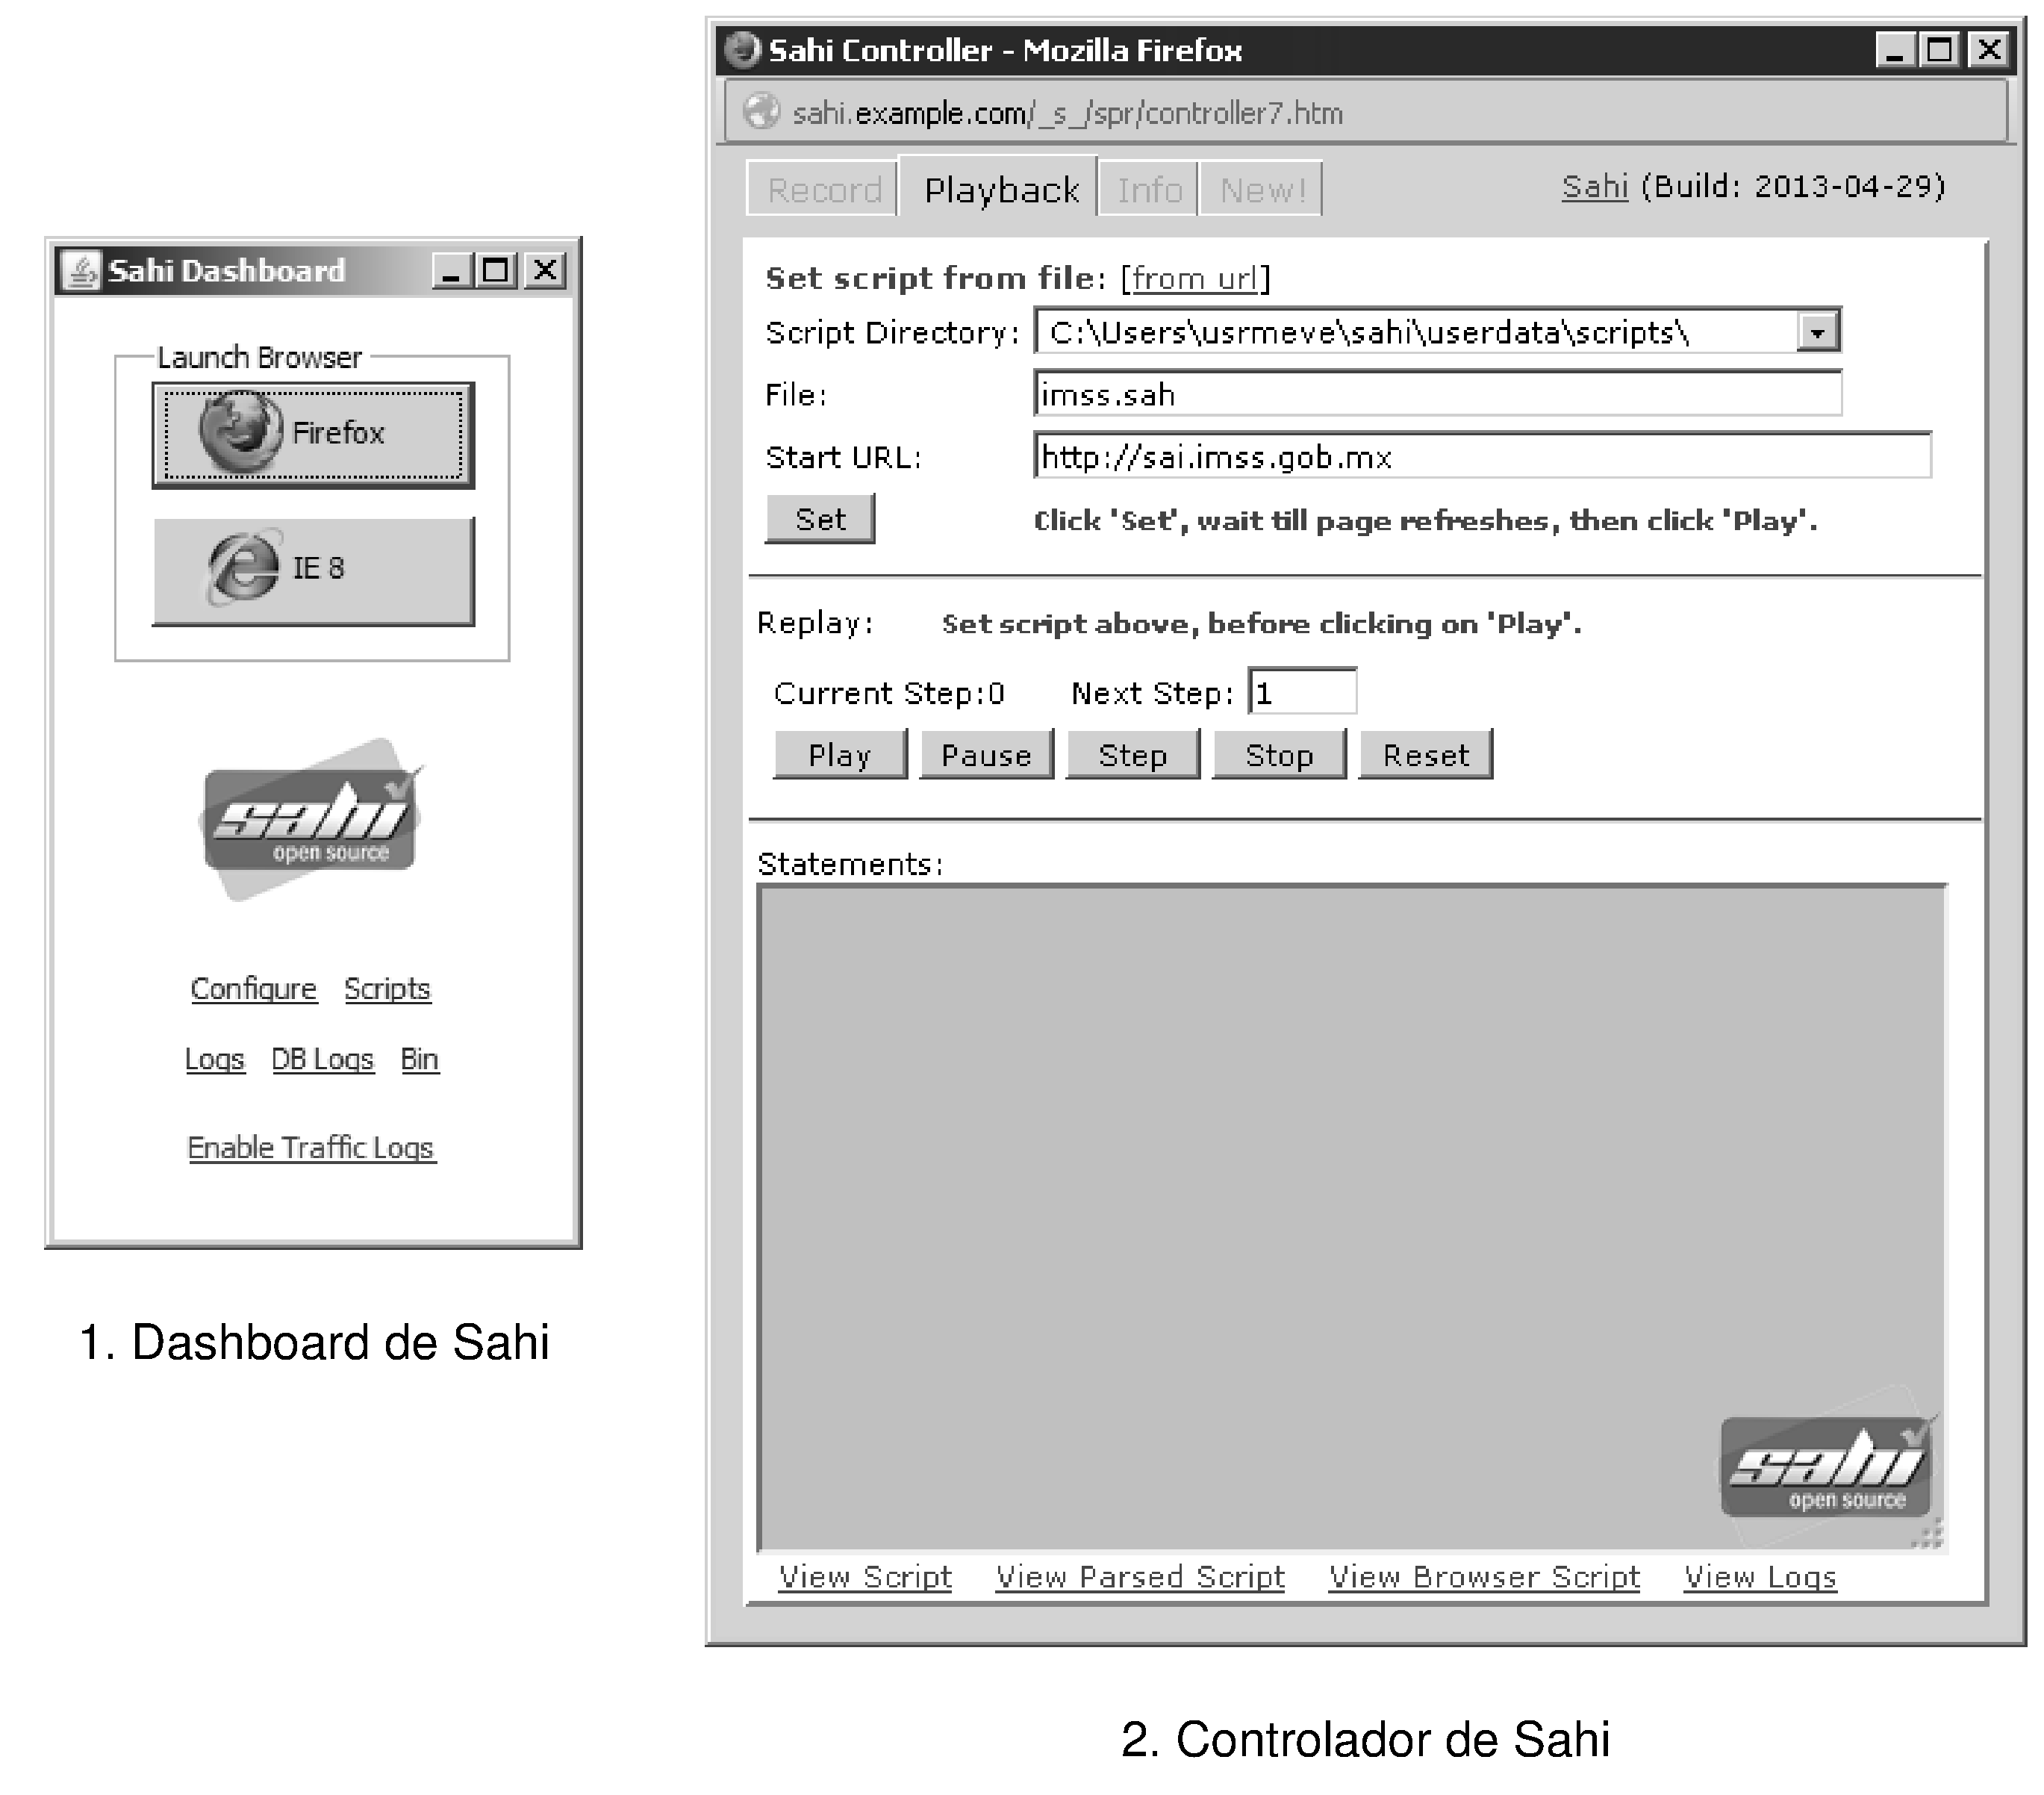
\includegraphics[scale=0.2]{ss-sahi}
		\caption{Interfaz de usuario de \textit{Sahi}.}
		\label{fig:ss-sahi}
	\end{figure}

	\item Iniciar el controlador de \textit{Sahi} y hacer los siguientes pasos (ver punto 2 de la Figura \ref{fig:ss-sahi}):
	\begin{enumerate}
		\item Seleccionar la rutina automatizada (contestar órdenes de reposición o verificación de órdenes de reposición)
		\item Ingresar la URL del Sistema de Abastecimiento
		\item Iniciar la ejecución.
	\end{enumerate}
\end{itemize}

\subsubsection{Interfaz web para la administración de órdenes de reposición contestadas}
La interfaz web descrita en este requerimiento (ver sección \ref{sec:req-web-ui}) fue elaborada a lo largo de la sección \ref{sec:web-portal}, en particular los servicios de acceso y autorización fueron mostrados en el apartado 1 de la sección \ref{sec:backend}, así mismo, la pantalla de acceso fue descrita en el apartado 1 de la sección \ref{sec:frontend}.\\
Cabe mencionar que la pantalla de acceso es la primera pantalla que muestra la interfaz web (ver Figura \ref{fig:ss-login}).
\begin{figure}[h]
	\centering
	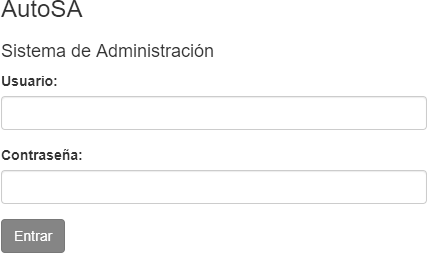
\includegraphics[scale=1.8]{ss-login}
	\caption{Captura de pantalla de acceso a la interfaz web.}
	\label{fig:ss-login}
\end{figure}

\subsubsection{Búsqueda de órdenes de reposición}
La pantalla para la búsqueda de órdenes de reposición es como se muestra al usuario la implementación del requerimiento de la sección \ref{sec:req-search}, la implementación de la pantalla y el comportamiento de están descritos en el apartado 4 de la sección \ref{sec:frontend}. Por otra parte, la implementación de los servicios web que consume la pantalla de búsqueda de órdenes de reposición es mostrada en el apartado 2 de la sección \ref{sec:backend}.\\
El la Figura \ref{fig:ss-search} se observa la captura de pantalla de búsqueda de órdenes de reposición.
\begin{figure}[h]
	\centering
	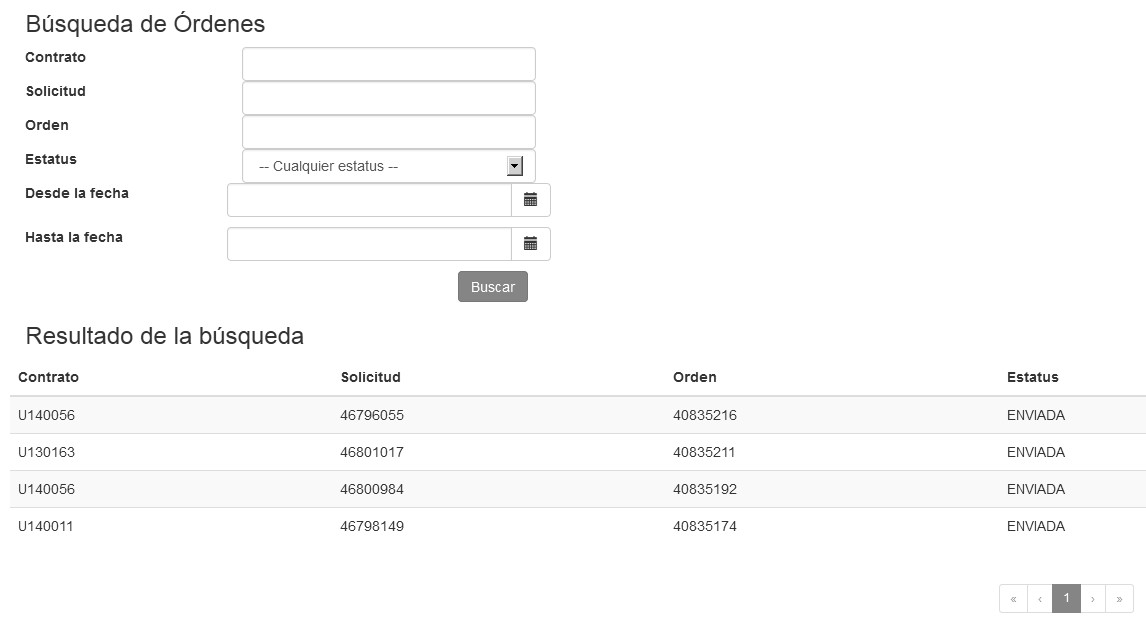
\includegraphics[scale=0.4]{ss-search}
	\caption{Captura de pantalla de búsqueda de órdenes de reposición.}
	\label{fig:ss-search}
\end{figure}

\subsubsection{Visualización y edición de una orden de reposición}
Los requerimientos para visualización y edición de una orden de reposición, requerimientos \ref{sec:req-show} y \ref{sec:req-update} respectivamente, son plasmados en los casos de uso CU-VISUALIZAR y CU-EDITAR (secciones \ref{cu-visualizar} y \ref{cu-editar} respectivamente). En la implementación y en la interfaz de usuario se utiliza la misma pantalla, como se muestra en la Figura \ref{fig:ss-edit}, esta vista es descrita en el apartado 5 de la sección \ref{sec:frontend}. La implementación de los servicios web que consume la pantalla son mostrados en el apartado 2 de la sección \ref{sec:backend}.
\begin{figure}[h]
	\centering
	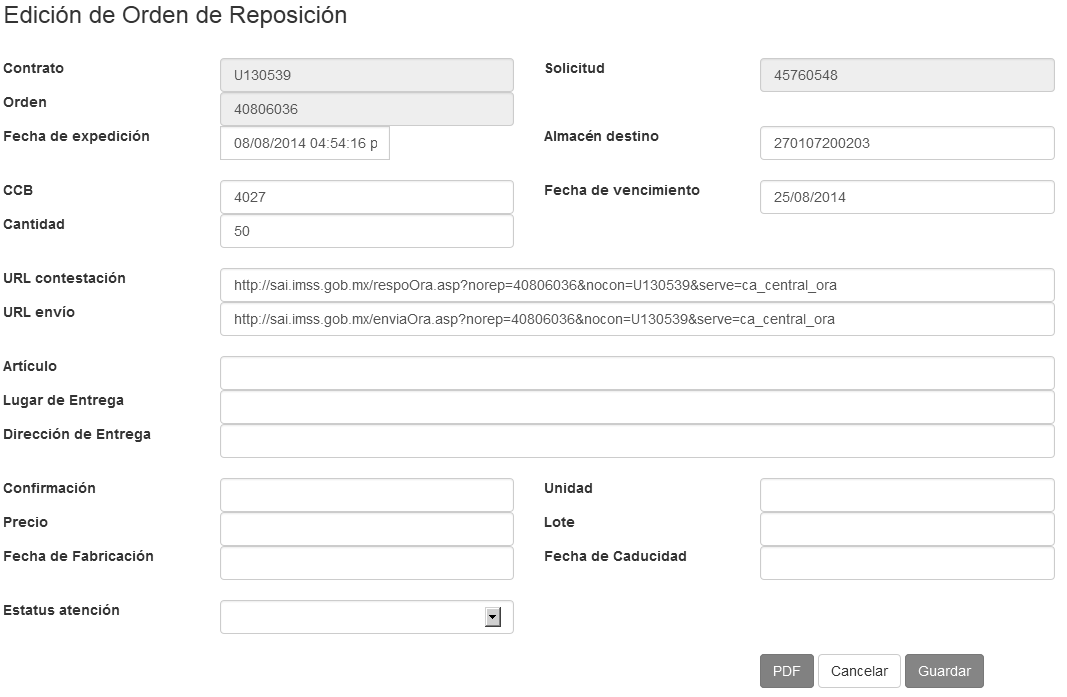
\includegraphics[scale=0.4]{ss-edit}
	\caption{Captura de pantalla de búsqueda de órdenes de reposición.}
	\label{fig:ss-edit}
\end{figure}

\subsubsection{Generación de reportes}
La generación de reportes cumple con los requerimientos de las secciones \ref{sec:req-rep-contestadas}, \ref{sec:req-rep-layout} y \ref{sec:req-rep-canceladas}; mismos que son englobados en el caso de uso CU-GENERAR-REPORTE (ver sección \ref{cu-generar-reporte}). La implementación de la generación de reportes está descrita en la sección \ref{sec:gen-repport} y, a su vez, los servicios web que exponen esta funcionalidad están en el apartado 2 de la sección \ref{sec:backend}. La vista que se muestra al usuario se encuentra en el apartado 2 de la sección \ref{sec:frontend}, en la Figura \ref{fig:ss-report} se observa la captura de pantalla como se muestra al usuario\footnote{Por acuerdo de confidencialidad no se puede mostrar el contenido de los reportes generados.}. 
	\begin{figure}[h]
		\centering
		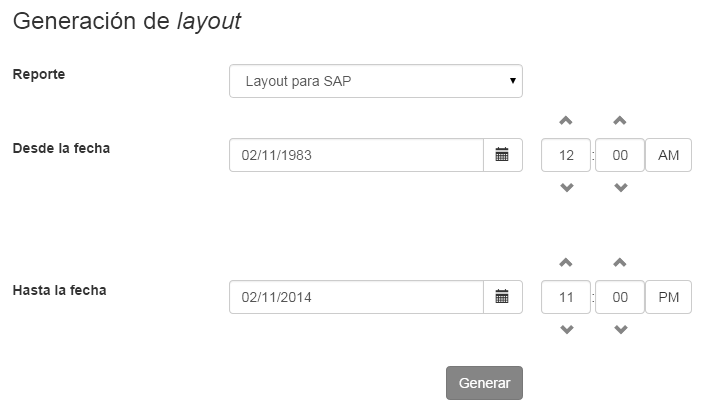
\includegraphics[scale=0.5]{ss-report}
		\caption{Captura de pantalla de generación de reportes.}
		\label{fig:ss-report}
	\end{figure}

\subsubsection{Actualización de catálogos y estatus de órdenes de reposición canceladas}
Los requerimientos \ref{sec:req-catalogos} y \ref{sec:req-canceladas} son modelados en el caso de eso CU-ACTUALIZAR-CATALOGO (ver sección \ref{cu-actualizar-catalogo}), la implementación de la actualización a los datos es dada en la sección \ref{sec:persistence-web}, y la implementación del servicio web se encuentra en el apartado 2 de la sección \ref{sec:backend}. La implementación de la vista está dada en el apartado 3 de la sección \ref{sec:frontend}, en la Figura \ref{fig:ss-catalog} se observa la captura de pantalla de la administración de catálogos\footnote{Por acuerdo de confidencialidad no se puede mostrar el contenido de los catálogos.}.
\begin{figure}[h]
	\centering
	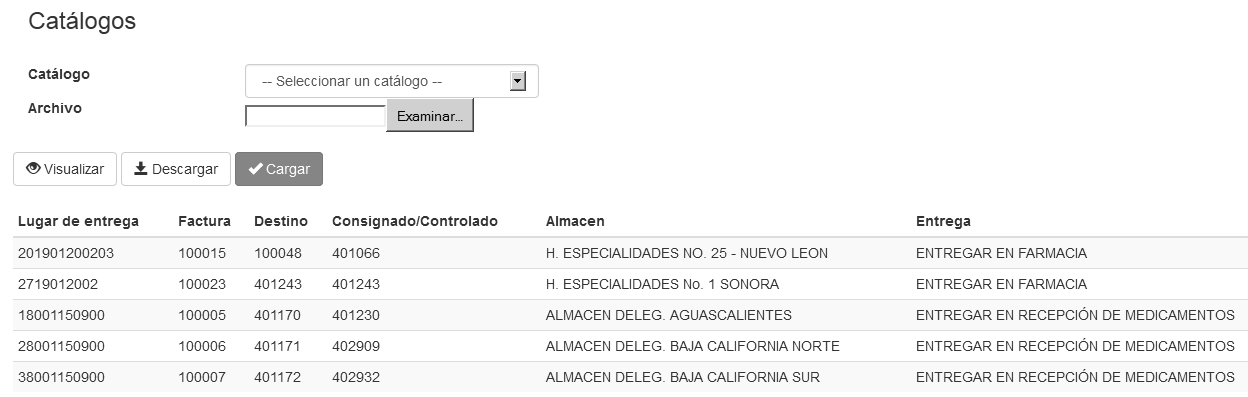
\includegraphics[scale=0.4]{ss-catalog}
	\caption{Captura de pantalla de administración de catálogos.}
	\label{fig:ss-catalog}
\end{figure}

\subsubsection{Navegación dentro de la interfaz web}
La implementación del requerimiento \ref{sec:req-nav-bar} es mostrada en la sección \ref{sec:frontend}, en la Figura \ref{fig:ss-nav-bar} se observa la captura de pantalla de la barra de navegación.
\begin{figure}[h]
	\centering
	
\includegraphics[scale=0.4]{ss-nav-bar}
	\caption{Captura de pantalla de la barra de navegación.}
	\label{fig:ss-nav-bar}
\end{figure}


\subsection{Cumplimiento de requerimientos no funcionales}
En la sección \ref{sec:nonfunctional-req} se enlistan los requerimientos no funcionales para el sistema AutoSA.

\subsubsection{Ejecución del Sistema AutoSA en los sistemas operativos más comunes.}
En la sección \ref{sec:java} se menciona que el lenguaje de programación Java es multiplataforma gracias a que el código escrito por los desarrolladores es traducido a \texttt{bytecode} y es este último el que ejecuta la máquina virtual de \textit{Java}. Existen implementaciones de robustas y ampliamente probadas de la Máquina Virtual de \textit{Java} para una gran variedad de sistemas operativos, es por esta razón que se decidió utilizar a \textit{Java} como el lenguaje de programación principal.

\subsubsection{Base de datos relacional \textit{SQL}}
Al principio del proyecto, la farmacéutica sentó que de ser necesaria una base de datos, el área encargada de las bases de datos de la farmacéutica sería quien daría la infraestructura y la base de datos provista sería relacional por lo que las rutinas DDL y DML de la sección \ref{sec:impl-db} y las consultas del módulo de persistencia (ver sección \ref{sec:persistence}) siguen los estándares \textit{SQL} mostrados en la sección \ref{sec:bd-r}.

\subsubsection{Uso de la herramienta \textit{Sahi} para automatizar interacción con Sistema de Abastecimiento}
En el cumplimiento de los requerimientos funcionales 1 y 2 de la sección anterior y en la sección \ref{sec:agente} se muestra la implementación del módulo \textbf{Agente} utilizando \textit{Sahi}.

\subsubsection{Las contraseñas de los usuarios para el acceso a la interfaz web deben ser almacenadas utilizando un algoritmo de cifrado}
En la sección \ref{sec:backend} se muestra la verificación y cifrado de la contraseña de un usuario.
